\documentclass[11pt]{article}
\usepackage[margin=1in]{geometry}
\usepackage{graphicx}
\usepackage{amsmath}
\usepackage{booktabs}
\usepackage{microtype}
\usepackage[hidelinks]{hyperref}

\renewcommand{\thesection}{S\arabic{section}}
\renewcommand{\thefigure}{S\arabic{figure}}
\renewcommand{\thetable}{S\arabic{table}}

\newcommand{\Faq}{\textit{F.~aquilonia}}
\newcommand{\Fpo}{\textit{F.~polyctena}}
\newcommand{\rsq}{\ensuremath{r^{2}}}

\title{\vspace{-3em}Supplementary Methods:\\
LD-based complexity reduction and the analysis of ancestry sorting}
\author{}
\date{}

\begin{document}
\maketitle
\vspace{-4em}

\noindent A recurring principle organises the procedures below. Markers in
linkage disequilibrium (LD) do not carry independent information, so the unit of
analysis throughout is the LD cluster rather than the marker; quantities are
measured per cluster, and statistical tests treat clusters, not markers, as
observations. Two further conventions follow from the same reasoning and are
stated where they arise: a variable that is to be tested as a predictor is never
also used to select the data, and a criterion whose stringency would otherwise
depend on cluster size is expressed as a rate rather than a count.

\section{Data}

\subsection{Samples}
Twenty hybrid populations between \Fpo{} and \Faq{} were sampled (164
individuals in total), together with allopatric reference individuals of both
parental species. \textit{Formica} wood ants are haplodiploid, so males are
haploid; this is relevant to the demographic modelling reported separately and
to the interpretation of within-population variation.

\subsection{Markers and ancestry polarisation}
Genotypes and per-marker ancestry information were taken from the DIEM output
for this dataset. Sites were restricted to those called as biallelic. For each
marker DIEM supplies a polarity and a diagnostic index (DI), the latter
measuring how informative the marker is about parental ancestry. Genotype
dosages at markers whose polarity indicated the opposite orientation were
replaced by $2-\text{dosage}$, so that after this step dosage is on a single,
consistent ancestry-oriented scale genome-wide. All later use of DI refers to
this per-marker diagnostic index.

\subsection{Frequency filtering and the two genotype matrices}
Minor allele frequencies were computed among the hybrid individuals only, and
markers retained at MAF $\ge 0.05$, giving 1{,}114{,}340 markers. Two genotype
matrices were then constructed over this same marker set. The first contains the
164 hybrid individuals only and is used for all LD estimation, clustering and
complexity reduction. The second additionally contains the parental reference
individuals and is used only where parental allele frequencies are required, for
example to orient ancestry or to compute between-species divergence. The
separation is deliberate: parental and hybrid individuals differ far more from
each other than hybrids differ among themselves, so including parents in the LD
computations would let between-species differentiation dominate every pairwise
LD estimate and obscure the within-hybrid-zone LD structure that the clustering
is designed to capture.

\section{Estimation of LD decay}

\subsection{Model and fitting}
LD decay was modelled per chromosome as
\begin{equation}
\rsq(d) \;=\; b + \frac{c-b}{1 + a\,d},
\end{equation}
where $d$ is physical distance in base pairs, $a$ is the decay rate, $b$ is the
long-range background level of \rsq{}, and $c$ is short-range \rsq{}. Background
LD was estimated from inter-chromosomal marker pairs, which are unlinked by
construction and therefore provide the appropriate baseline. Within each
chromosome the curve was fitted across twenty sliding windows with 50\% overlap,
sampling up to 5{,}000 marker pairs per window stratified across twenty distance
classes so that short and long distances are represented comparably; \rsq{} was
summarised at its 0.95 quantile, and the per-window fits were aggregated over
the central 95\% of windows to limit the influence of individual outlying
windows.

\subsection{Allele-frequency filtering during fitting}
Only pairs in which both markers exceeded MAF 0.1 contributed to the background
and decay-curve fits. Pairs involving rare alleles mechanically depress \rsq{}
irrespective of true linkage, and including them biases the fitted $a$, $b$ and
$c$. This restriction applies to curve fitting alone: the stored pairwise LD
edge lists retain all markers, so no marker is lost from the downstream
clustering.

\subsection{Decay rate, chromosome size, and window sizes}
Decay rates vary systematically with chromosome length, so a robust regression
of $a$ on chromosome size was fitted genome-wide, allowing decay behaviour to be
described consistently across chromosomes of very different length. For a target
relative LD threshold $\rho$, the corresponding physical distance follows from
the fitted curve as
\begin{equation}
d \;=\; \frac{\rho}{a\,(1-\rho)} ,
\end{equation}
which is how all distance-based windows below are obtained. Anchoring distances
in each chromosome's own fitted decay curve, rather than in a fixed base-pair
window or a fixed \rsq{} cutoff, is what makes a single threshold behave
comparably across chromosomes with different background LD.

\subsection{Local LD support}
For each marker a measure of local LD support, $\mathrm{ld}_w$, was computed as
the median \rsq{} between that marker and its neighbours within the window
corresponding to $\rho = 0.95$. It summarises how strongly a marker is embedded
in local LD. Its practical value is that it is a per-marker quantity read
directly from the LD data: unlike a recombination rate, which must be
interpolated from a genetic map, and unlike the decay rate $a$, which is fitted
per window, $\mathrm{ld}_w$ requires no interpolation and is defined at the
resolution of the individual marker.

Because reduced recombination elevates local LD, $\mathrm{ld}_w$ reflects the
local recombination environment. Treating the least-recombining regions,
defined as the lowest quantiles of map-based recombination rate, as the target,
both $\mathrm{ld}_w$ and the window-level decay rate $a$ discriminate them well:
across the lowest 5\%, 10\% and 25\% of windows, $a$ achieves areas under the
receiver-operating-characteristic curve of 0.91 to 0.98 and $\mathrm{ld}_w$ of
0.73 to 0.86 (Fig.~\ref{fig:roc}). The decay rate is the stronger predictor,
as expected of a window-level summary, but $\mathrm{ld}_w$ retains the
resolution and directness required for a per-marker decision. Such a
directly-measured LD statistic is also informative where a pedigree-based
recombination estimate is not: in this cross roughly two thirds of
adjacent-marker intervals contain no observed recombinant, so the direct
estimate is uninformative over most of its range. The correspondence is also
visible directly along the chromosome: $\mathrm{ld}_w$ is elevated exactly over
each low-recombination region, where both the decay rate and the map-based rate
are reduced (Fig.~\ref{fig:tracks}). $\mathrm{ld}_w$ is used below to identify
clusters for reconsideration in Stage~2.

\begin{figure}[h]
\centering
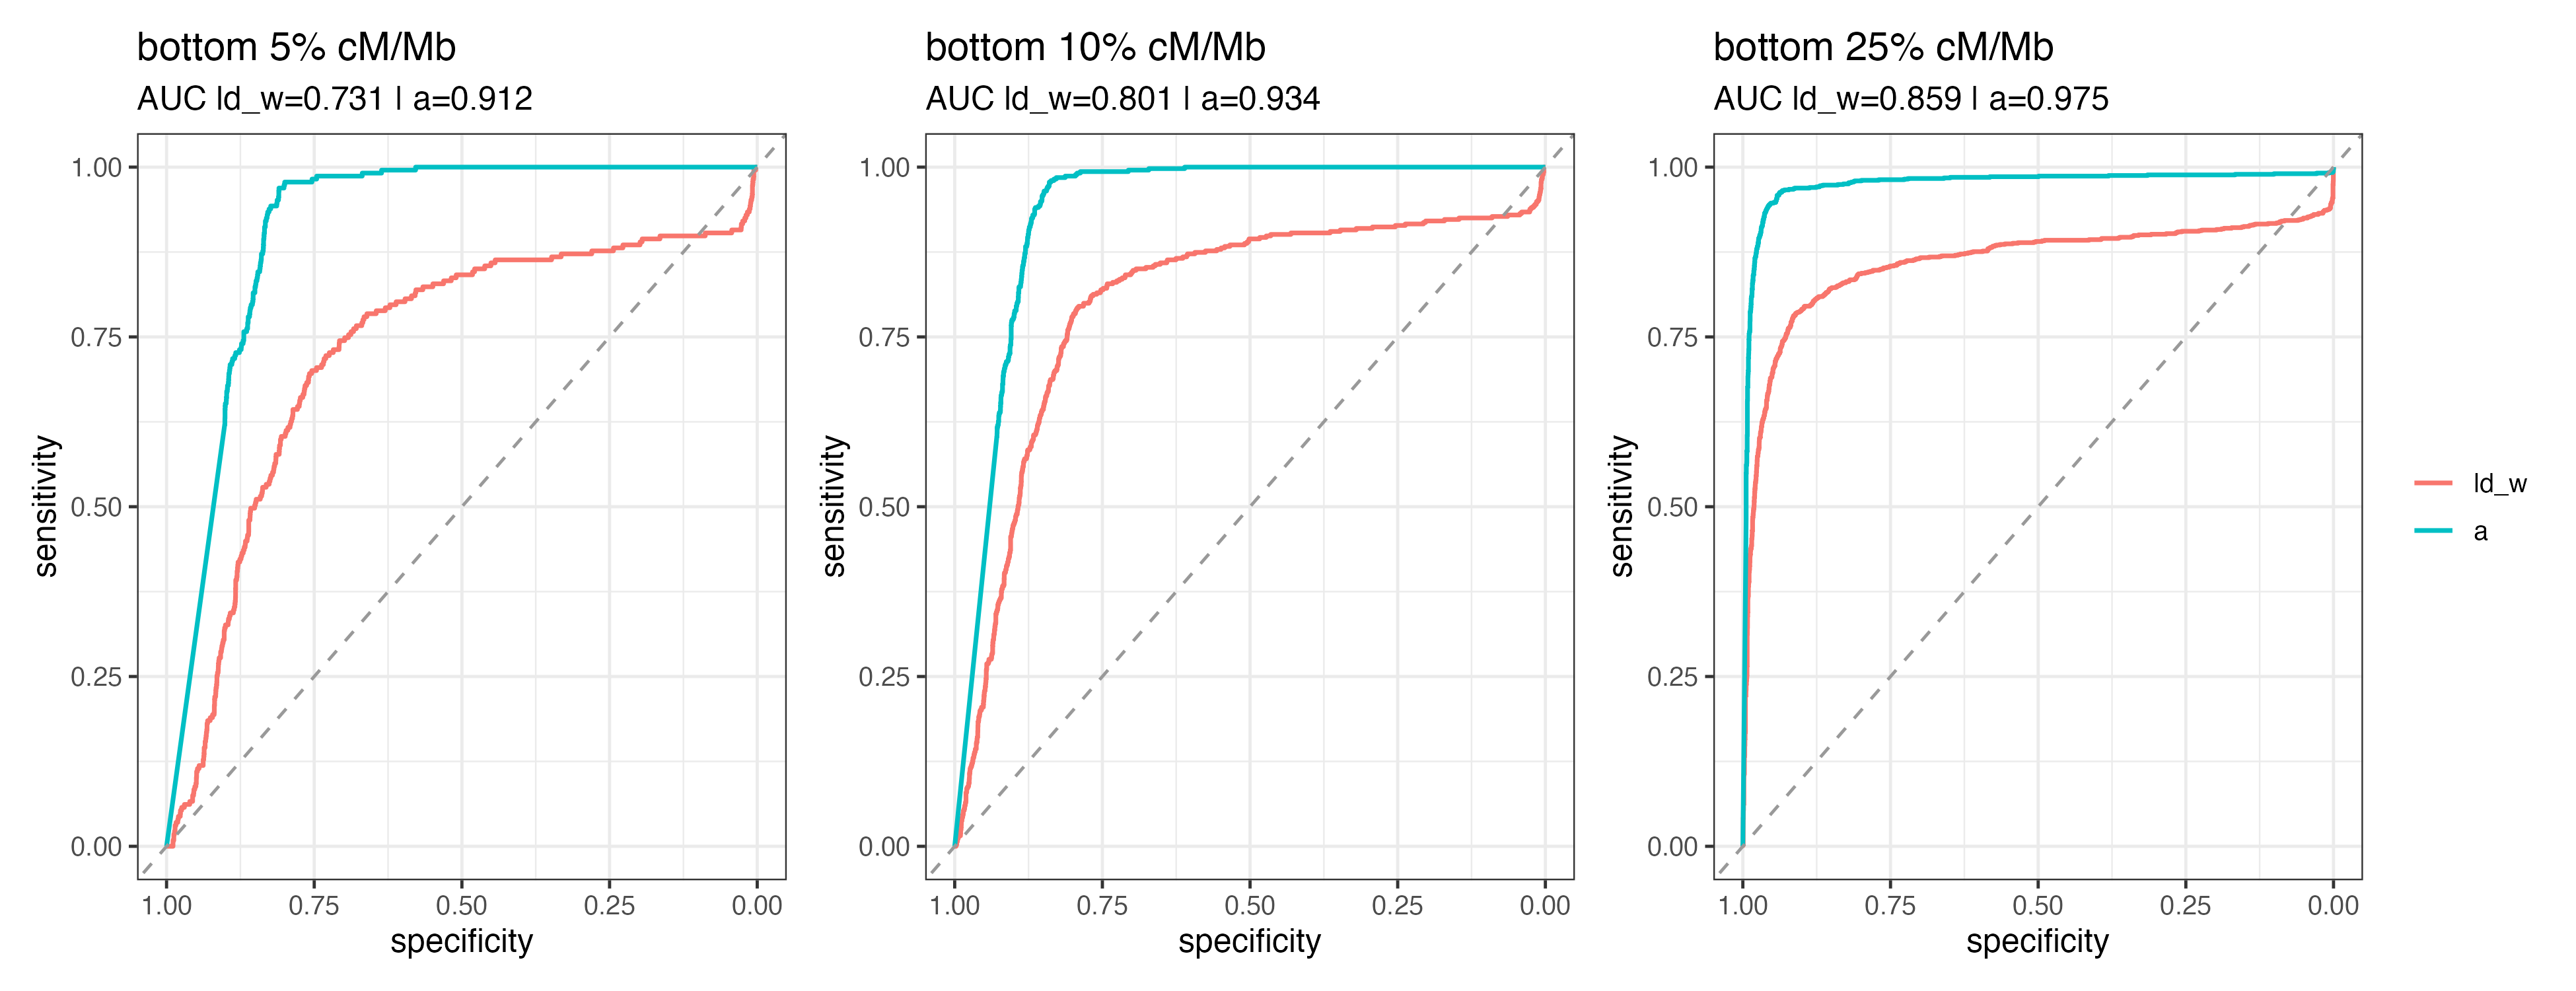
\includegraphics[width=0.95\textwidth]{../Figures/p_roc_low_recombination.png}
\caption{Discrimination of low-recombination regions by local LD support
($\mathrm{ld}_w$) and by the window-level decay rate ($a$), against
map-based recombination rate, at three definitions of ``low recombination''
(the lowest 5\%, 10\% and 25\% of windows). Both are effective; the decay rate
is stronger, while $\mathrm{ld}_w$ is defined per marker and requires no
interpolation.}
\label{fig:roc}
\end{figure}

\begin{figure}[h]
\centering
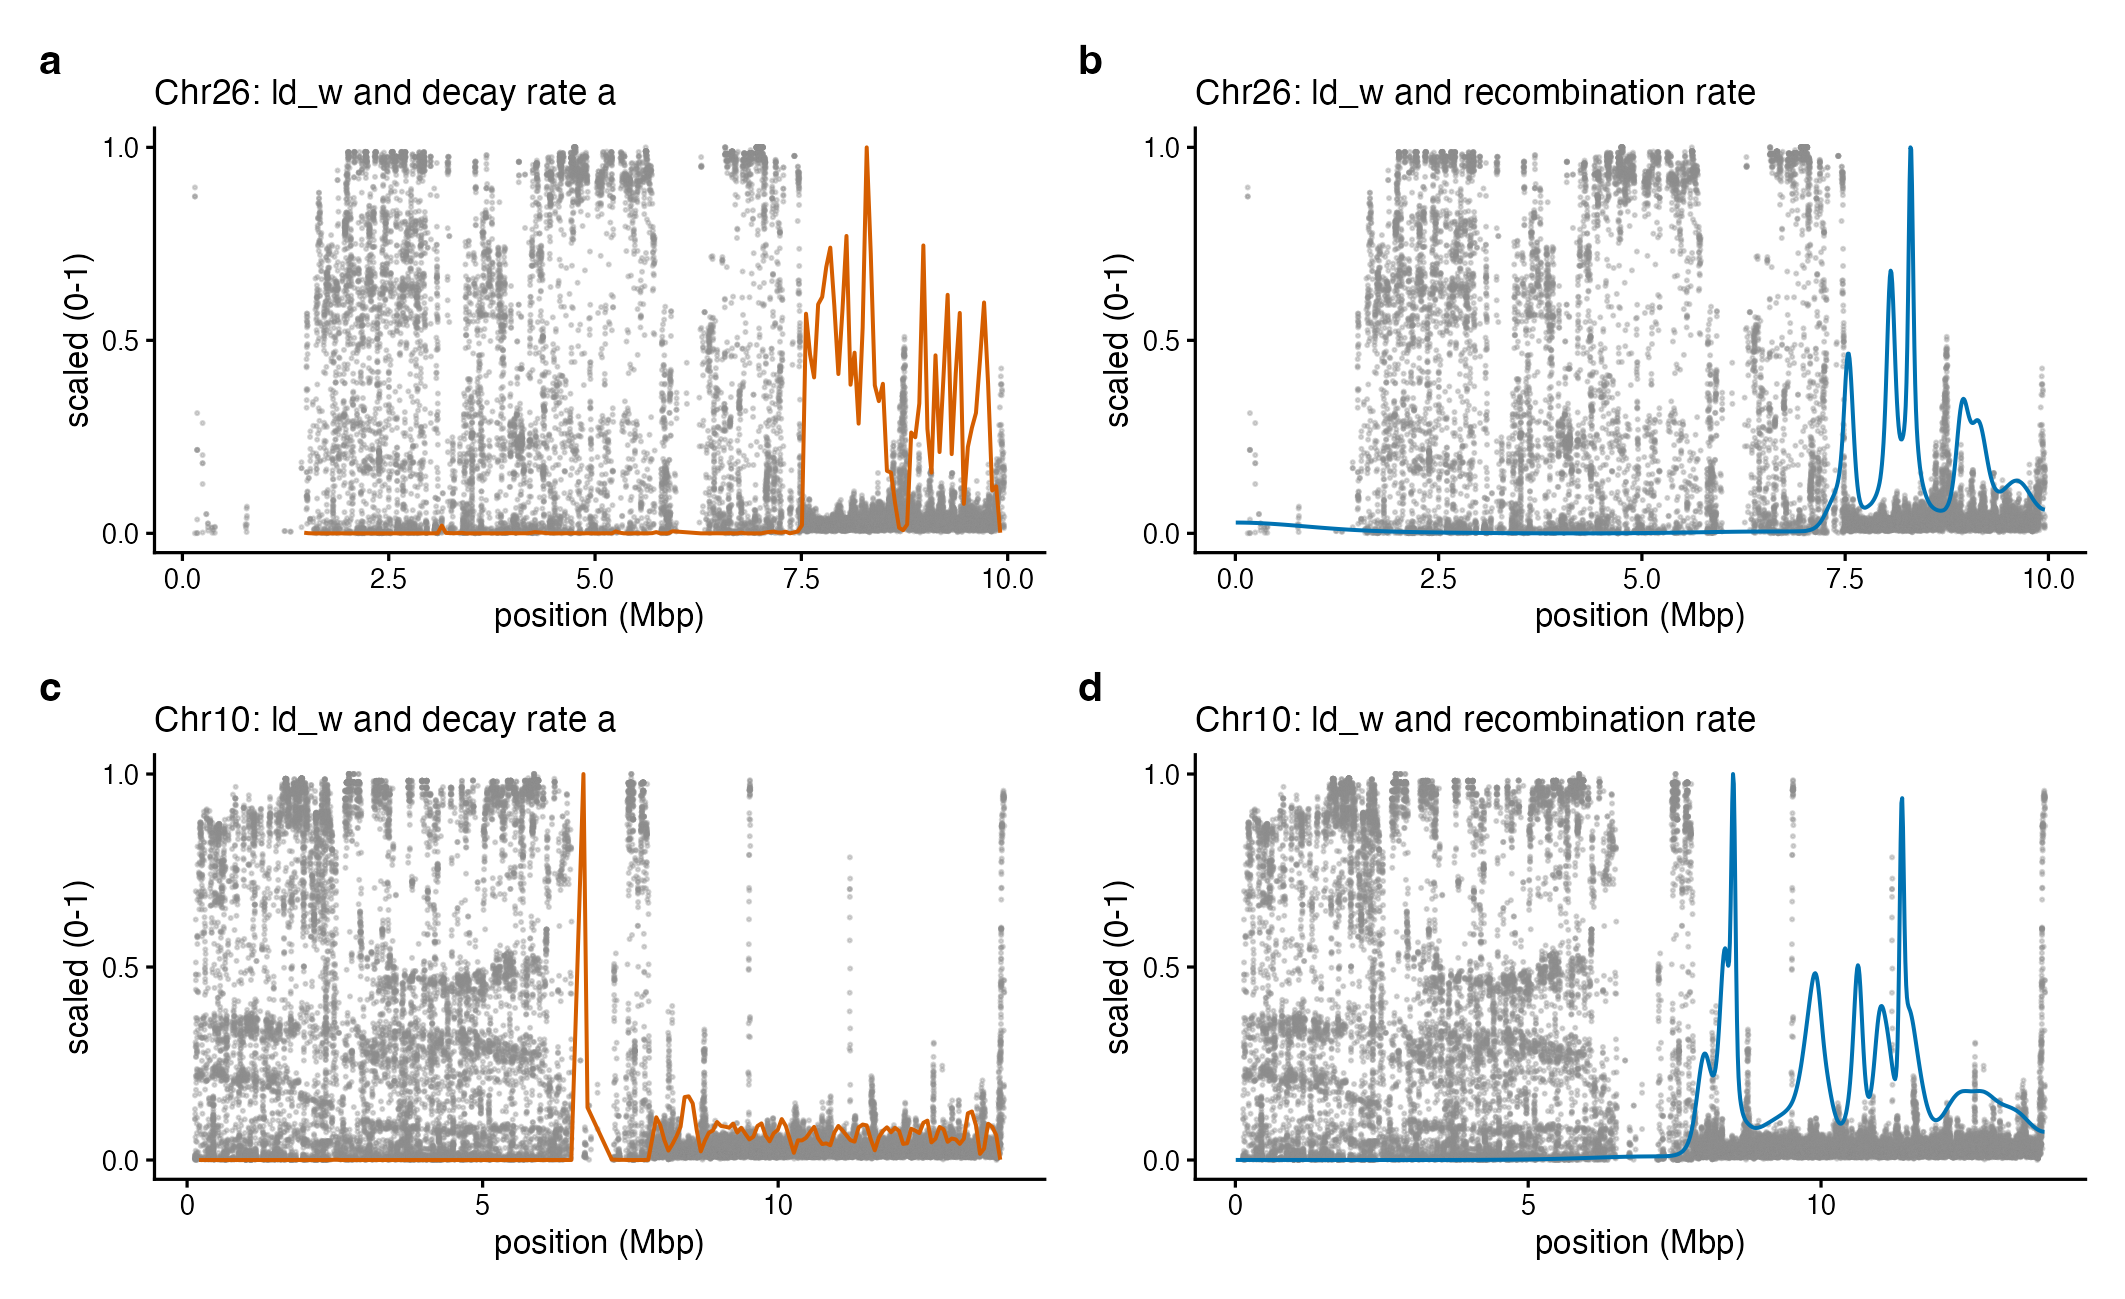
\includegraphics[width=\textwidth]{../Figures/ld_tracks_chr26_chr10.png}
\caption{Per-marker local LD support ($\mathrm{ld}_w$, grey points) along two
example chromosomes, each with a pronounced low-recombination region, shown
against the window-level decay rate $a$ (orange, left column) and the map-based
recombination rate (blue, right column); every series is min-max scaled.
$\mathrm{ld}_w$ is elevated across each low-recombination region, where both $a$
and the recombination rate are reduced. Note the directions: $a$ is a decay
rate, so $a$ and the recombination rate are positive correlates of each other,
whereas $\mathrm{ld}_w$ is their inverse.}
\label{fig:tracks}
\end{figure}

\section{Complexity reduction: one partition, two projections}

\subsection{Rationale}
LD pruning and the construction of consensus genotypes are usually treated as
separate procedures, but they answer the same question: what is the finest
partition of markers that can no longer be distinguished statistically, and
therefore constitutes an independent unit in these data? Once that partition is
fixed, two projections of it are useful. Selecting one representative marker per
cluster gives an LD-pruned marker set. Collapsing each cluster to a single consensus
dosage gives an expected multi-locus genotype (eMLG) per cluster. Both are
produced here from a single clustering pass, so the two representations always
refer to the same underlying units.

\subsection{What a cluster represents, and why it is not a haplotype block}
A biallelic marker carries exactly one bipartition of the sampled chromosomes: it
divides them into two groups and can encode nothing further. Where the local
genealogy contains more than two segregating lineages, mutations falling on
different branches define \emph{different} bipartitions. Markers arising on the
same branch are carried by the same set of lineages and are therefore perfectly
correlated, in the absence of recombination, recurrent mutation and missing data;
markers arising on different branches are correlated only partially, according to
how those branches are related.

Clustering on linkage disequilibrium therefore groups markers by the partition of
individuals they report, not by their position, and two consequences follow.
First, clusters need not partition the chromosome: where several branches
segregate in one region, the markers tagging each are physically interleaved, so
the resulting clusters overlap along the sequence. The distance restriction
applied below keeps clusters local, but locality is not spatial exclusivity.
Second, because \rsq{} is sensitive to allele frequency, two markers tagging
\emph{nested} branches can show complete association on a frequency-independent
measure and yet a low \rsq{}; clustering on \rsq{} accordingly separates nested
branches, which is precisely the situation in which a single interval contains
several overlapping clusters.

For these reasons we avoid the term haplotype block. A block, in its usual sense,
is a contiguous stretch of limited haplotype diversity with defined boundaries,
implicitly reflecting a single genealogy, and it partitions the sequence. The
units here are instead sets of markers reporting the same partition of
individuals, several of which may occupy the same interval. The reduction
performed below is over information content---which split of the sample a marker
reports---rather than over physical space.

This is also what makes a consensus genotype meaningful. Averaging markers that
report the same partition reinforces the dosage of that partition, whereas
averaging across partitions would blur distinct splits. The complete-linkage
requirement in Stage~1 and the pairwise correlation floor in Stage~2 both exist to
prevent that.

\subsection{Stage 1: local LD clusters}
The clustering threshold was derived, per chromosome, from that chromosome's own
fitted decay curve at $\rho = 0.5$, its half-decay point, rather than from a
fixed \rsq{} cutoff applied genome-wide. The threshold was deliberately not
allowed to vary further \emph{within} a chromosome: a region with unusually slow
local decay, such as a centromere or an inversion, is precisely where markers
are most redundant and pruning should be most aggressive, so adapting the
threshold to tolerate high local LD there would defeat the purpose.

Clustering proceeded in two steps on the precomputed pairwise LD edge list.
Markers were first grouped into connected components of the thresholded sparse
graph, which is inexpensive; each component was then refined into
complete-linkage sub-clusters by hierarchical clustering on the dense sub-matrix
of \rsq{} values within it. The second step is necessary because single linkage
alone permits chaining through a mosaic LD pattern: two markers that are
uncorrelated with each other can be joined through an intermediate marker
correlated with both, and would then be wrongly treated as redundant. Complete
linkage instead requires every pairwise \rsq{} within a final cluster to clear
the threshold.

The representative of each cluster was taken to be the marker with the highest
median \rsq{} to the remaining cluster members. This is preferred to selecting
the marker most strongly correlated with the cluster's mean genotype, because
the latter is sensitive to allele-coding direction: a genuinely central marker
coded on the opposite allele correlates negatively with the mean and would be
passed over. Since \rsq{} ignores sign, the median-\rsq{} criterion does not have
this failure mode.

\subsection{Why Stage 1 is conservative, and how Stage 2 resolves it}
The pairwise LD edge list is built within a sliding window, so pairs of markers
farther apart than that window were never evaluated; in the clustering they
behave as though $\rsq = 0$. Single linkage tolerates this, because a chain of
overlapping windows still connects distant markers. Complete linkage does not:
a genuine single cluster wider than the window is fragmented into several
clusters purely because the unevaluated pairs default to zero. The window is
sized from average decay behaviour to reach a high $\rho$, which covers typical
regions comfortably, but slowly-recombining regions decay far more slowly than
that average and are where fragmentation is expected.

Stage~2 addresses this after the fact rather than by changing Stage~1. Candidate
clusters are compared directly from genotypes, with no window restriction, and
are selected for reconsideration using Stage~1's own cluster boundaries. Markers
are deliberately not pre-split by their local LD before clustering: doing so
severs real clusters exactly at the selection boundary, whereas selecting whole
clusters leaves genuine clusters intact.

\subsection{Stage 2: quality-gated merging}
A Stage-1 cluster was flagged for reconsideration if any of its members exceeded
$\mathrm{ld}_w > 0.025$, or if the cluster contained at least five markers. The
$\mathrm{ld}_w$ criterion follows directly from what the statistic measures: a
marker with low local LD support is by definition weakly correlated with its
neighbours, and is therefore already close to independent and would not merge
with anything. Restricting the reconsideration to markers with appreciable local
support concentrates this comparatively expensive step exactly where a merge is
possible, without omitting merges elsewhere. The second criterion is a separate
route in, for clusters that have already grown to at least five markers---and so
demonstrably do cluster---but whose local support is only moderate, which would
otherwise pass through unmerged. Flagged clusters were
then merged by a distance-restricted, average-linkage dynamic tree cut that
accepts each candidate merge only while two quality conditions hold: the
consensus genotype must survive hard-calling, quantified as
$\mathrm{score}_{\mathrm{eMLG}}(x) = \mathrm{cor}(\mathrm{round}(x),x)^2 \ge
0.80$, which is the property downstream LD statistics require of a consensus;
and the two sides being merged must themselves be correlated, at pairwise
$\rsq \ge 0.2$. The two conditions are not redundant. Fidelity is a property of
the resulting consensus, and once a cluster is large that consensus is dominated
by the markers already in it, so appending a few further markers changes the
score very little whether or not they report the same partition. The fidelity
criterion is therefore least discriminating precisely where clusters are
largest, and the pairwise requirement is what prevents an essentially
uncorrelated marker from being absorbed there. Because merging proceeds only
while both conditions hold, this stage cannot over-merge regardless of how
permissively clusters were flagged.

The distance restriction was applied in genetic rather than physical units, at
0.5~cM, using the linkage map. Physical distance is a poor and sometimes
misleading proxy for recombination distance in this genome: cluster pairs more
than a megabase apart can be at essentially zero genetic distance, while others
only a few hundred kilobases apart span several centimorgans. A genetic
threshold also behaves correctly on exceptional chromosomes, where a slower
local recombination rate gives 0.5~cM a proportionally larger physical span,
instead of clipping a genuine cluster to a distance calibrated on typical
chromosomes.

\subsection{Outputs and conventions}
The procedure returns both projections of the partition: one representative
marker per cluster, and a consensus dosage for clusters of at least five markers
($\mathrm{min\_n\_loci\_eMLG} = 5$). The size threshold is a computational
limit on consensus construction, not a redefinition of the unit: clusters below
it remain valid units and retain their pruning representative, and the pruned
marker set is unchanged by this setting. Clustering results were written to a
file whose name encodes the parameters used, so that analyses depending on a
particular clustering cannot silently be run against a different one.

\begin{figure}[h]
\centering
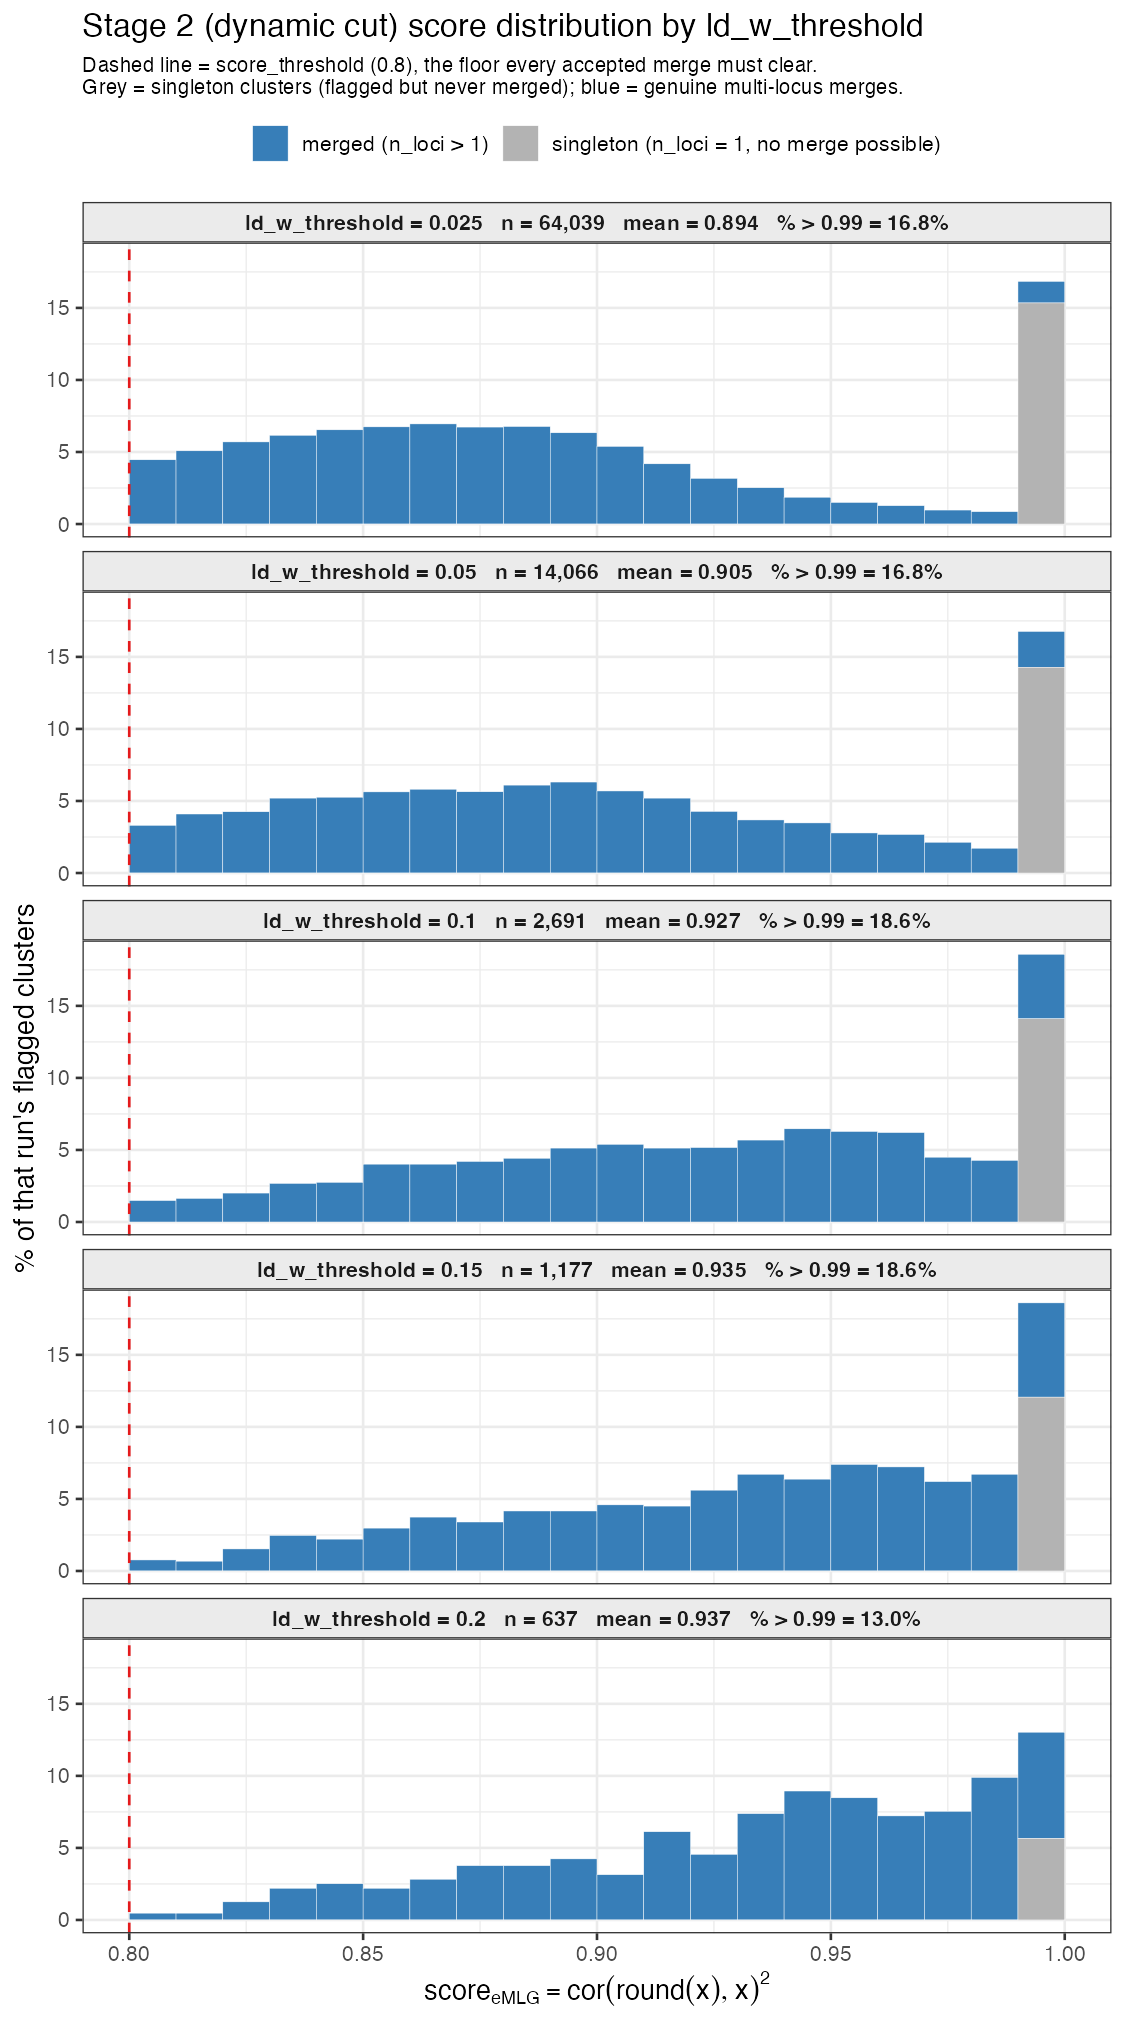
\includegraphics[width=0.95\textwidth]{../Figures/eMLG_score_histograms_by_threshold.png}
\caption{Distribution of consensus round-trip fidelity
($\mathrm{score}_{\mathrm{eMLG}}$) across flagged clusters at five
$\mathrm{ld}_w$ flagging thresholds, with clusters separated into single-marker
clusters, for which no merge was possible, and genuine multi-marker merges. The
separation matters for interpreting mass near the upper limit, which at
permissive thresholds consists largely of isolated markers with no correlated
neighbour rather than of merges stopping early.}
\label{fig:score}
\end{figure}

\begin{figure}[h]
\centering
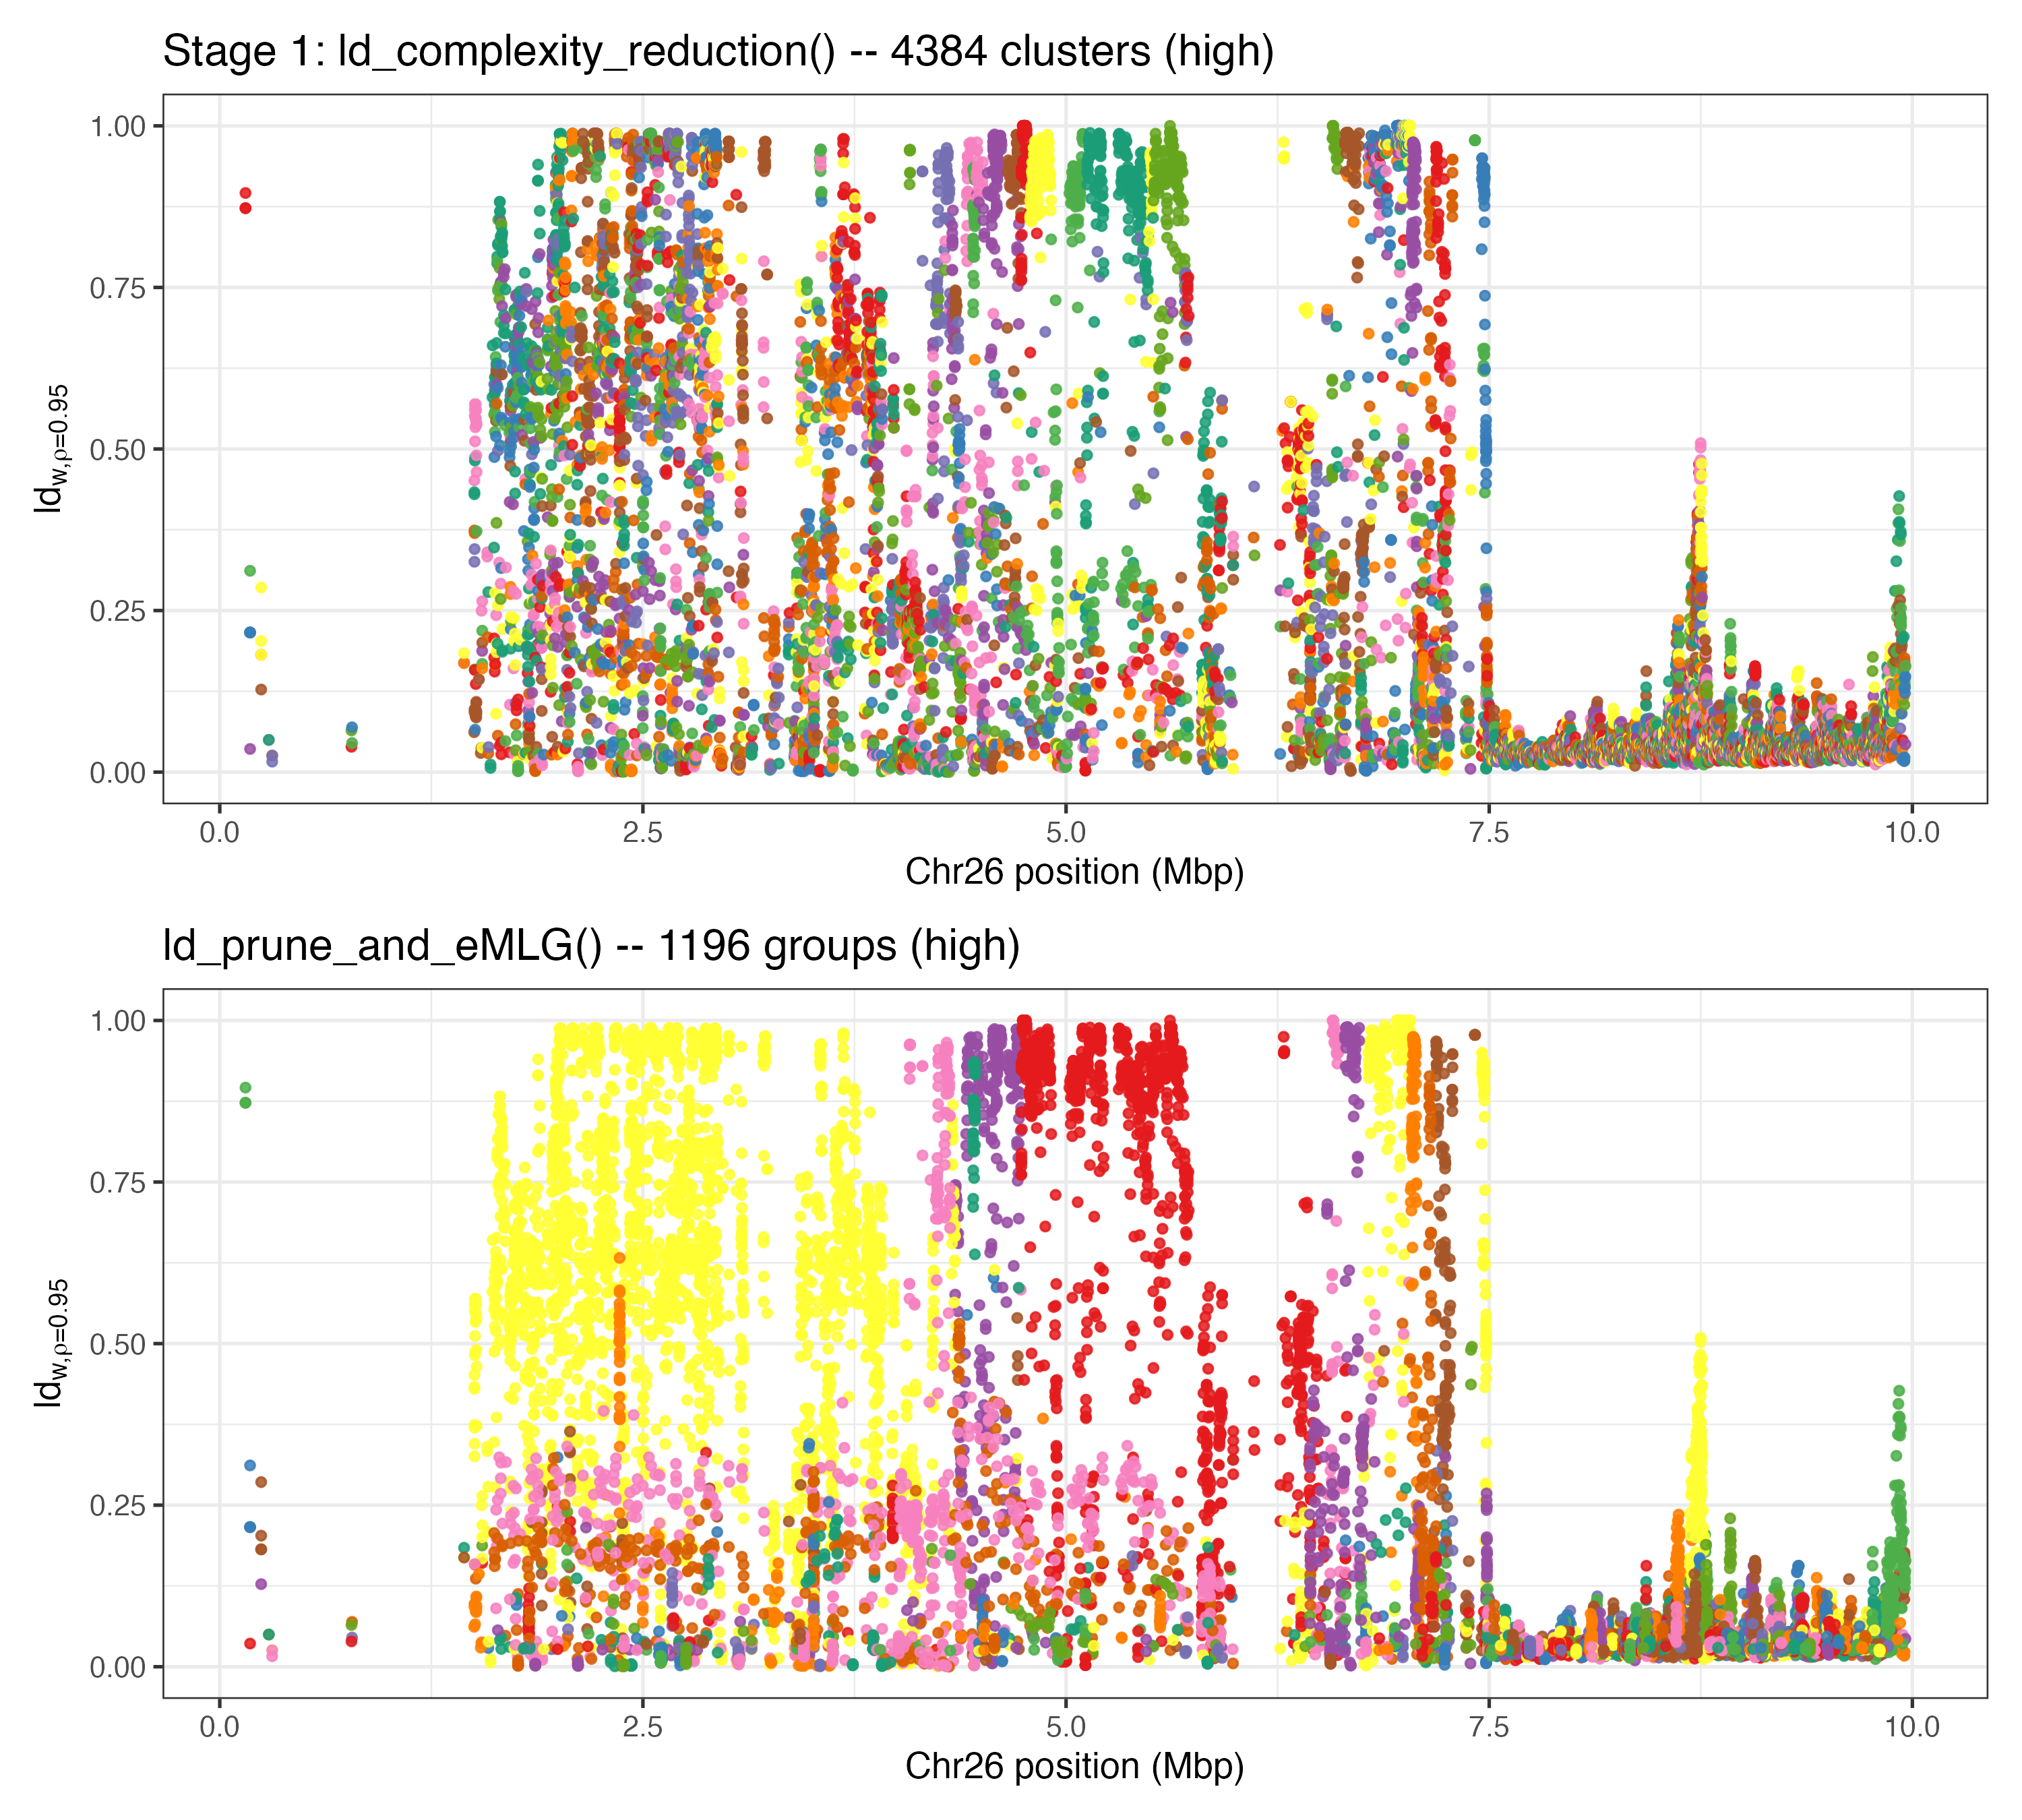
\includegraphics[width=0.8\textwidth]{../Figures/Chr26_stage1_vs_combined_high.png}
\caption{Stage~1 clustering compared with the combined two-stage result for
Chr26, restricted to markers with high local LD support. Fragmented Stage-1
clusters within each low-recombination region are consolidated into single
coherent clusters per physical LD peak, which is the intended effect of Stage~2.}
\label{fig:prune}
\end{figure}

\section{Sorting statistics}

\subsection{Orientation and near-fixation}
The question these statistics address is whether parental ancestry sorts
\emph{predictably} across the replicate hybrid populations---the same parental
allele approaching fixation repeatedly---or in directions that vary among
populations. For each locus, dosage was oriented into an \Faq-allele frequency
using the parental reference samples: the sign of the difference in allele
frequency between the two parental species defines which allele is counted, and
loci at which the parents do not differ have no defined orientation. Each hybrid
population was then classified as near-fixed toward \Faq{} if its oriented
frequency was at least $1-\theta$, near-fixed toward \Fpo{} if it was at most
$\theta$, and unsorted otherwise, with $\theta = 0.15$. This tolerance
interacts with population sample size, since a population of few diploid
individuals can only realise a coarse grid of frequencies, and was therefore
held constant across all analyses rather than tuned per analysis.

\subsection{Decomposition and classification}
Let $n_{\mathrm{obs}}$ be the number of populations with data and a defined
orientation, and $n_{\mathrm{aqu}}$ and $n_{\mathrm{pol}}$ the numbers near-fixed
in each direction. Sorting was decomposed as
\begin{equation}
\underbrace{\frac{n_{\mathrm{aqu}}+n_{\mathrm{pol}}}{n_{\mathrm{obs}}}}_{\text{prop\_fixed}}
=\;\Bigl|\underbrace{\tfrac{n_{\mathrm{aqu}}-n_{\mathrm{pol}}}{n_{\mathrm{obs}}}}_{\text{uni}}\Bigr|
\;+\;\underbrace{\frac{2\min(n_{\mathrm{aqu}},n_{\mathrm{pol}})}{n_{\mathrm{obs}}}}_{\text{bi}} ,
\end{equation}
separating the extent to which populations fixed in a consistent direction from
the extent to which they fixed in opposing directions. A single threshold
$\tau = 0.5$ on these quantities classifies each locus: unidirectional (toward
one parent) when $|\mathrm{uni}| \ge \mathrm{bi}$ and $|\mathrm{uni}| \ge \tau$,
bidirectional when $\mathrm{bi} > |\mathrm{uni}|$ and $\mathrm{bi} \ge \tau$, and
unsorted otherwise. Because all three quantities are fractions of the population
panel, the same threshold is directly comparable between individual markers and
aggregated clusters, and genome-wide summaries are simple tallies over units.

\subsection{Test of directional predictability}
Among the $n_{\mathrm{fixed}}$ populations that near-fixed in either direction,
predictability was tested as
\begin{equation}
n_{\mathrm{aqu}} \sim \mathrm{Binomial}(n_{\mathrm{fixed}},\, 0.5),
\end{equation}
two-sided and exact, computed only where $n_{\mathrm{fixed}} \ge 5$, with
Benjamini--Hochberg adjustment across tested loci. The null probability of $0.5$
encodes the symmetric expectation, under which populations fix in either
direction with equal chance. A per-locus alternative, in which each locus is
tested against its own mean ancestry across the hybrid populations, is not
appropriate here: that expectation is itself a direct function of the outcome
being tested, so it absorbs the very signal of interest. Genome-wide mean \Faq{}
ancestry at diagnostic loci is close to $0.5$, so the symmetric null is also the
empirically correct one.

The descriptive classification and the test are reported as separate
quantities throughout. The classification states how much and in which direction
a unit sorted, at a fixed threshold; the test states whether the direction
departs from the random-direction expectation. They answer different questions
and are never combined into a single label.

\subsection{The polymorphism gate}
Near-fixation in the hybrid populations is evidence of \emph{sorting} only if the
locus was segregating in the founding admixture. Analyses were therefore
restricted to loci polymorphic in the parents, using the pooled parental minor
allele frequency---computed from pooled allele counts across all parental
individuals and folded to the minor allele---with a threshold of $0.15$.

The gate is deliberately placed on parental allele frequency rather than on the
diagnostic index. DI is a predictor to be tested in later analyses, against
recombination, cluster size, climate association and the direction of sorting.
Selecting loci on DI would truncate its range, attenuating every one of those
relationships, and would make the question of whether DI predicts sorting
circular. Parental allele frequency instead performs the role a gate should
perform here: it removes loci that were already near-monomorphic in the founding
pool, where near-fixation in the hybrids reflects the starting condition rather
than a sorting event, while leaving DI free to vary across its full range.

We note that the magnitude of sorting and the unsorted/bidirectional/
unidirectional classification are invariant to which allele is designated
\Faq{}, since exchanging the labels exchanges $n_{\mathrm{aqu}}$ and
$n_{\mathrm{pol}}$ without altering their sum or their minimum. Only the parental
\emph{direction} depends on the orientation, and is therefore interpretable only
where the parental samples differ.

\subsection{Testing at the level of clusters}
The same statistic was applied to the eMLG consensus genotypes so that each LD
cluster contributes one test rather than one test per constituent marker. Stored
consensus genotypes cover clusters of at least five markers; for the remaining
clusters containing a sorted marker, consensus genotypes were constructed by the
identical procedure, so that every cluster is tested at whatever resolution its
size permits and none is represented only by its individual markers.

Testing a cluster requires parental as well as hybrid consensus genotypes, since
orientation is defined from the parents. The parental consensus was constructed
using the reference-marker choice and per-marker flip decisions derived from the
hybrid genotypes, rather than recomputed on the parental individuals alone.
Recomputing them on a small and strongly differentiated parental sample can
select a different reference marker and flip a different subset of markers,
which would place the hybrid and parental consensus genotypes on opposite
orientations for any marker where the two choices disagree, without any error
being raised.

The diagnostic index of a cluster was taken as the maximum across its member
markers, so that a cluster is excluded by a DI criterion only if none of its
members is ancestry-informative. Using the representative marker alone would
exclude clusters whose informative markers lie elsewhere in the cluster.

\subsection{Distinguishing absence of signal from dilution}
A cluster may contain a marker that sorts individually and yet not sort once its
members are aggregated. Two situations produce this, and they were separated
using the same round-trip fidelity measure that governs merging: a coherent
cluster whose consensus is faithful and genuinely does not sort, versus a
heterogeneous cluster in which averaging across dissimilar members dilutes a real
signal. Blocks falling below the fidelity floor used during clustering were
flagged for separate consideration.

\section{Genomic architecture}

\subsection{Genomic covariates}
Recombination rate was assigned per marker by linear interpolation of the
linkage map, in centimorgans per megabase. From the parental allele frequencies
$p_{\mathrm{aqu}}$ and $p_{\mathrm{pol}}$ we computed within-species diversity as
the mean of the two species' expected heterozygosities, absolute divergence as
\begin{equation}
d_{xy} = p_{\mathrm{aqu}}(1-p_{\mathrm{pol}}) + p_{\mathrm{pol}}(1-p_{\mathrm{aqu}}),
\end{equation}
and relative differentiation $F_{\mathrm{ST}}$ in the standard form
$(H_T - H_S)/H_T$. Reporting relative and absolute measures alongside diversity
is what allows a peak of differentiation caused by reduced within-species
diversity to be distinguished from one caused by genuinely elevated divergence,
a distinction that a relative measure alone cannot make.

\subsection{Marker-level versus unit-level summaries}
Sorting was summarised across recombination deciles twice: once treating each
independent unit as one observation, using the pruning representatives, and once
on a random sample of individual markers. The comparison is diagnostic rather
than decorative. Adjacent markers within a low-recombination region report the
same underlying event, so a relationship that is present at marker level and
absent at unit level reflects the spatial redundancy of markers rather than a
property of the units themselves.

\subsection{Cluster size as collider and as confounder}
Block size occupies a different causal position in different questions here, and
is handled differently in each; we state this explicitly because the same
variable is deliberately treated in opposite ways.

When relating recombination to sorting, cluster size is a consequence of both
recombination and local diversity, and therefore a collider. It is excluded from
those models: conditioning on it induces an apparent association between
recombination and sorting that is not otherwise present.

When relating climate-association outlier status to the diagnostic index
(Section~\ref{sec:climate}), cluster size is a confounder. It independently
predicts DI genome-wide, and it is also required by any criterion that counts
significant members within a cluster. It is therefore adjusted for in those models.

\subsection{Direction of sorting versus architecture}
To ask whether genomic architecture predicts the \emph{direction} of sorting
beyond the diagnostic index, the direction of unidirectionally sorted units was
modelled by logistic regression on standardised diagnostic index, log
recombination rate, pooled parental allele frequency and log cluster size, fitted
across units. Any recombination term here is an association: under neutrality a
non-recombining autosomal region does not experience stronger drift than its
surroundings, so attributing such a term to linked selection requires an
explicit demographic null, which is evaluated separately.

\section{Association with climate}
\label{sec:climate}

\subsection{Genotype--environment association}
Per-population allele frequencies were associated with per-population climate
covariates---two principal components of the climate variables, constant within
a population---using BayPass, with evidence reported as Bayes factors on the
deciban scale. Eight runs were performed, crossing two population sets, the two
climate axes, and two treatments of the among-population covariance matrix. In
one treatment the covariance matrix is estimated beforehand from the LD-pruned
marker set under the core model and supplied to the association run; in the
other it is estimated internally from the full marker set. Estimating it from
the pruned set is preferable in principle, because linkage disequilibrium among
markers otherwise inflates the apparent covariance among populations; running
both allows the sensitivity of any result to that choice to be reported.

The association output carries no marker identifier, only a row index into the
genotype file supplied to the program. Results were therefore matched to markers
positionally, and every import is guarded by assertions that the number of rows
equals the number of markers and that the index is a strictly increasing
sequence, so that a mismatch caused by regenerating the inputs raises an error
rather than silently assigning evidence to the wrong markers.

\subsection{Ancestry as a potential confounder}
Sorting is by definition the fixation of parental ancestry, so a climate axis
that is itself correlated with genome-wide ancestry could appear to co-localise
with sorting for structural rather than ecological reasons. We therefore
estimated ancestry directly: for each population, the mean \Faq-allele frequency
across ancestry-diagnostic markers, oriented from the parental samples, and
examined its correlation with each climate axis. Because a correlation across
twenty populations can rest on very few of them, the correlation was recomputed
with individual populations removed to identify any that carried it.

Two controls follow from this and are applied throughout. First, conditioning on
the among-population covariance matrix absorbs the shared population structure
with which such an axis is correlated. Second, the population set excluding the
population identified as carrying the ancestry--climate correlation was taken as
the primary analysis, with the full set retained as a comparator. Results are
reported across all eight runs so that dependence on either choice is visible.

\subsection{Association strength per cluster}
Each cluster's climate association was summarised as its \emph{significance
rate}: the proportion of its member markers reaching the Bayes factor threshold.
A rate is used rather than a count of significant members because a count makes
eligibility depend on cluster size. A cluster of nine markers would need more than
half of its members to be individually significant in order to reach a count of
five, whereas a cluster of ninety needs only a small fraction; the same nominal
criterion is therefore far stricter for small clusters. This cannot be repaired by
conditioning on cluster size, because the resulting eligibility is a hard,
strongly non-linear function of size rather than a smooth trend, and the
adjustment would have to extrapolate across a range in which one outcome cannot
occur at all. Expressing association as a rate removes the dependence by
construction, and cluster size is retained as a covariate for its independent
effects.

Because a rate is estimated imprecisely when a cluster contains few markers,
results are reported across nested size strata rather than pooled: all clusters,
those with at least twenty markers, and those with at least fifty. Reporting the
strata together makes the dependence of any estimate on measurement precision in
the predictor explicit.

\subsection{Testing at the level of clusters}
Blocks are the units of observation, as elsewhere. For the diagnostic-index
outcome, the quantity modelled is the proportion of a cluster's members that are
ancestry-informative, with each cluster contributing one observation. A
size-weighted model with an overdispersion correction is reported alongside it as
a check. The corresponding marker-level model is not used as the primary
analysis: it treats markers within a cluster as independent trials, whereas they
are in linkage disequilibrium by construction, which understates the standard
errors substantially. The relationship between climate association and the
sorting classification was tested in the same way, with the cluster's
classification as the outcome.

\section{Among-population disequilibrium between unlinked clusters}
\label{sec:intrinsic}

\subsection{Rationale}
The per-locus sorting statistics ask, locus by locus, whether ancestry fixes in a
consistent direction across the replicate populations; they say nothing about
whether \emph{pairs} of loci fix in a coordinated way. An intrinsic incompatibility
between two loci---a Dobzhansky--Muller interaction, in which particular
combinations of parental ancestry are unfit---acts on the joint ancestry of the
pair rather than on either locus alone. Across independent, non-migrating
replicate populations such an interaction has a distinctive signature: the two
loci repeatedly fix compatible ancestry in the same direction, so their allele
frequencies covary across populations more than either does with an arbitrary
third locus. For loci that are not physically linked this covariance cannot be
produced by recombinational linkage, and under drift alone independent replicates
sort unlinked loci independently, so its neutral expectation is close to zero.
Elevated among-population two-locus disequilibrium between unlinked clusters is
therefore the pair-level quantity that an intrinsic incompatibility would raise,
complementary to the per-locus sorting measured above.

\subsection{Units and the restriction to unlinked pairs}
The units are the eMLG consensus genotypes, as in the sorting analysis, so that
each LD cluster contributes once and physically redundant markers are not counted
repeatedly. Pairs were formed only between clusters on different chromosomes. This
is the restriction that makes the test specific: same-chromosome pairs can carry
disequilibrium through linkage irrespective of any interaction, whereas
between-chromosome pairs cannot, so an association there must arise from correlated
sorting rather than from proximity. Same-chromosome pairs were retained not as
tests but as an internal reference---the disequilibrium expected where linkage is
present---against which the unlinked pairs are read.

\subsection{The polymorphism gate}
As in the sorting analysis, clusters were restricted to those polymorphic in the
founding admixture, using the pooled parental minor allele frequency at a threshold
of $0.15$. The reasoning carries over on both counts. A cluster carries
interpretable ancestry information, and an among-population ancestry covariance is
defined for it, only if it was segregating in the parents; and placing the gate on
parental allele frequency, rather than on the diagnostic index or on any property
of how the hybrids sorted, keeps the selection off every quantity the screen then
measures---the same separation of selection from tested variable applied throughout.

\subsection{Decomposition and the two-stage screen}
Two-locus disequilibrium was partitioned into within- and among-population
components following Ohta's decomposition, computed from unphased genotypes. The
component of interest is the among-population one---the variance across populations
of the product of subpopulation allele frequencies relative to the total---which is
what correlated among-population sorting elevates. It is reported together with the
within-population component and with the disequilibrium of the averaged population,
so that a genuine among-population covariance can be distinguished from a systematic
within-population association. The exact decomposition counts joint genotype classes
and so requires integer dosages; it was therefore evaluated on the hard-called
consensus, whereas the screening proxy below, which uses allele frequencies only,
was computed from the continuous consensus without rounding.

The pairs between differentiated clusters number in the hundreds of millions, the
great majority carrying no association, so the exact decomposition was not evaluated
for every pair. A cheap proxy was computed for all of them---the correlation across
populations of the per-population mean consensus dosage, denoted $R_{\mathrm{st}}$
---and the exact decomposition was evaluated only for pairs whose absolute
correlation reached $0.7$. The proxy is a linear, allele-frequency-based
approximation of the very among-population covariance the exact statistic measures,
so the pre-filter selects pairs on the target quantity itself rather than on an
unrelated criterion; and because it is a deterministic function of the
per-population frequencies, it can be applied identically to observed and to
simulated genotypes, keeping the conditioning matched whenever the screen is
repeated against a null.

\subsection{Status of the screen}
With only twenty populations the among-population correlation is estimated
imprecisely, and it is in any case dominated by the single genome-wide gradient in
ancestry that runs through all diagnostic loci; the screen is accordingly
descriptive. It ranks pairs and yields the distribution of among-population
disequilibrium, but does not by itself identify incompatibilities. Candidate
interactions are those whose among-population disequilibrium exceeds the
recombination-matched neutral expectation, obtained by applying the identical
pre-filter and decomposition to genotypes simulated under the demographic null
described separately, with the same-chromosome pairs serving as the concurrent
within-data reference. The screen is implemented so that this null comparison
reuses the same procedure unchanged.

\section{Software and reproducibility}

LD decay estimation, complexity reduction, consensus genotype construction and
the associated diagnostics are implemented in the \texttt{LDscnR} package; the
analyses described above are scripted in the project repository, one script per
stage.

Two conventions support reproducibility. Clustering results and any output whose
content depends on an analysis threshold are written to filenames that encode the
parameters used, so that alternative settings coexist rather than overwrite one
another and no analysis can silently be run against a clustering it was not built
on. Second, the computationally expensive intermediate---the parental consensus
genotypes---is cached, and is by construction independent of the downstream
thresholds, so that re-analysis under a different criterion does not require it
to be recomputed.

\begin{table}[h]
\centering
\caption{Parameter settings used throughout.}
\label{tab:params}
\small
\begin{tabular}{lll}
\toprule
Stage & Parameter & Value \\
\midrule
Marker set & site type & biallelic \\
 & MAF among hybrids & $\ge 0.05$ (1{,}114{,}340 markers) \\
\midrule
LD decay & background pairs & inter-chromosomal, 5{,}000 markers \\
 & windows per chromosome & 20, 50\% overlap \\
 & pairs per window & $\le 5{,}000$, 20 distance strata \\
 & \rsq{} quantile & 0.95 \\
 & MAF for curve fitting & $> 0.1$ (both members) \\
 & robust aggregation & central 95\% of windows \\
 & local support $\mathrm{ld}_w$ & median \rsq{} within $\rho = 0.95$ window \\
\midrule
Stage 1 & clustering threshold & per chromosome at $\rho = 0.5$ \\
 & linkage & components, then complete linkage \\
 & representative & highest median \rsq{} to cluster \\
\midrule
Stage 2 & flagging & $\mathrm{ld}_w > 0.025$ or $\ge 5$ markers \\
 & consensus fidelity floor & $\mathrm{score}_{\mathrm{eMLG}} \ge 0.80$ \\
 & pairwise correlation floor & $\rsq \ge 0.2$ \\
 & distance restriction & 0.5 cM (genetic map) \\
 & consensus size threshold & $\ge 5$ markers \\
\midrule
Sorting & near-fixation tolerance & 0.15 \\
 & classification threshold & 0.5 \\
 & null probability & 0.5 \\
 & minimum fixed populations & 5 \\
 & parental MAF gate & $\ge 0.15$ (pooled counts) \\
 & cluster diagnostic index & maximum across members \\
 & multiple testing & Benjamini--Hochberg \\
\midrule
Climate & evidence threshold & $\mathrm{BF(dB)} \ge 15$ \\
 & runs & 2 population sets $\times$ 2 axes $\times$ 2 covariance settings \\
 & diagnostic-index criterion & DI $> -25$ \\
 & size strata & all, $\ge 20$, $\ge 50$ markers \\
\midrule
Intrinsic LD & unit & eMLG consensus (hard-called) \\
 & pair restriction & different chromosomes \\
 & cluster gate & parental MAF $\ge 0.15$ \\
 & screening proxy & among-population dosage correlation $R_{\mathrm{st}}$ \\
 & pre-filter threshold & $|R_{\mathrm{st}}| \ge 0.7$ \\
 & disequilibrium & Ohta within/among-population components \\
\bottomrule
\end{tabular}
\end{table}

\end{document}
